\documentclass[12pt]{article}
\usepackage{amscd,amssymb,amsthm,amsxtra,exscale,latexsym,verbatim,paralist}
\usepackage{mathrsfs}
\usepackage[T1]{fontenc}
\usepackage{newtxmath,newtxtext}
\usepackage[left = 2cm, top = 2cm, bottom = 2cm, right = 2cm]{geometry}

\usepackage{hyperref}
\usepackage{tikz}
\usetikzlibrary{patterns}

\newcommand{\XB}{\color{black}}
\newcommand{\XBB}{\color{blue}}
\newcommand{\XV}{\color{violet}}
\newcommand{\XR}{\color{red}}
\newcommand{\ds}{\displaystyle}

\setlength{\parindent}{0pt} 
\setlength{\parskip}{\baselineskip}

\begin{document}

\title{\textbf{MTH385}: History of Mathematics - Final Essay}
\date{\today}
\author{\XV\textit{\large{\href{https://github.com/casonk}{Cason Konzer}}}\XB}

\maketitle

\hrulefill

\newpage

\section{Introduction}

\hspace{5mm}
Within this sort essay I will recount the history of the mathematical topics: 
Hyperbolic Geometry and Russell's Paradox.
The choice of topics stems from an interest in the artistic application of 
Hyperbolic Geometry and the logical contradiction present in Russell's Paradox. 
For each topic we will discuss in brief the inventor(s), idea(s), and context of their creation. 

\section{Hyperbolic Geometry}

\hspace{5mm}
The Euclid's propositions about lines, angles, and circles form the traditionally taught 
Euclidean geometry dearest to our hearts.

The postulates are as follows. \textbf{[12]} 

\begin{enumerate}
  \item To draw a straight line from any point to any point.
  \item To produce a finite straight line continuously in a straight line.
  \item To describe a circle with any center and distance.
  \item That all right angles are equal to one another.
  \item That, if a straight line falling on two straight lines make the interior angles
  on the same side less than two right angles, the two straight lines, if produced
  indefinitely, meet on that side on which are the angles less than the
  two right angles.
\end{enumerate}

The constraint on Euclidean geometry follows from the $5^{th}$ (parallel) postulate and when relaxed, 
holding all else equal, one enters the realm of non-euclidean geometry. 
A rephrasing of this postulate is as follows; Given a line $ L $ and a point $ P $ not on $ L $, 
there is exactly one line through $ P $ that does not intersect $ L $.
One may consider first a tighter constraint, such that there is absolutely no line 
through $ P $ that does not intersect $ L $, an elliptic (spherical) geometry. 
In a similar manner, a relaxation follows such that there exists multiple lines 
through $ P $ that do not intersect $ L $, a hyperbolic geometry of our concern. \textbf{[7]} 

\hspace{5mm}
The first word of these ideas are recollected in a letter from Gauss to Taurinus in 1824, 
``The assumption that the sum of the three angles [of a triangle] is smaller than 180° leads to a geometry 
which is quite different from our (euclidean) geometry, but which is in itself completely consistent.'' 
Though Guass did not publish his ideas, possibly due to fear of criticizing the work of Euclid, 
and the beginning of mathematical literature in hyperbolic geometry start with the work of Lobachevsky in 1829. 
Lobachevsky defines a natural unit for distance in hyperbolic space and then in 1930 conjectures that if we were to live 
in such a hyperbolic space, then our solar system is extremely small, computed at the time with an incorrect estimate of the parallax of Sirius.  
It was not long after, 1832, that J. Bolyai independently published ideas on non-euclidean geometry. \textbf{[8]} 

\hspace{5mm}
It is know that Guass was friends with the teacher, Bartles, of Lobachevsky, the father F. Bolyai, of J. Bolyai. 
As a result, many a historians have speculated that that the independent discoveries were not novel, but rather guided by Gauss. 
There is no evidence to support this claim, and yet other claims in its support have been debunked.
With this said it is indeed without a doubt that Gauss' work influenced the evolution of hyperbolic geometry in his theory of curved surfaces. 
The importance of the work of these two was not realized in due time, but rather the importance revolved around advancements in 1968 from
Riemann's theory of higher dimensional curved manifolds, and Beltrami's work on relating two-dimensional hyperbolic geometry to the 
study of suitable surfaces of constant negative curvature and the introduction of an n-dimensional pseudogeometry following that of the pseduosphere. \textbf{[8]} 
Three years later, after attending a seminar on Lobachevsky's geometry by Weiersreauss in 1870, Klein reinterpreted Beltrami's work in terms of projective geometry, 
which followed previous work from Cayley in 1859, of which is now refered to as the Klein-Beltrami (projective disk) model.
In a similar fashion, circa 1968, Beltrami obtained the conformal disk model known to Reimann and extended it to a half-space model 
of which the two-dimensional case have been previously discovered by Liouville. \textbf{[8]} \textbf{[11]} 

\hspace{5mm}
Poincaré took up the work on the half-space (upper half-plane) model from Liouville and Beltrami then in 1882. 
Of which he continued to work on making major contribution then in 1882 and additionally in 1887. 
As a result of his advancements in conjunction with the may others pushing the field, 
there is two models commonly referred to attributed to him in hyperbolic geometry, 
the Poincaré upper half-plane model as mentioned a prior, and the Poincaré disk model. \textbf{[8]} \textbf{[11]} 
The Poincaré disk model was later taken up by the artist commonly know to mathematical enthusiasts, M.C. Escher. \textbf{[2]} 
We conclude this section with a famous work of his utilizing such model below. 

\begin{center}
  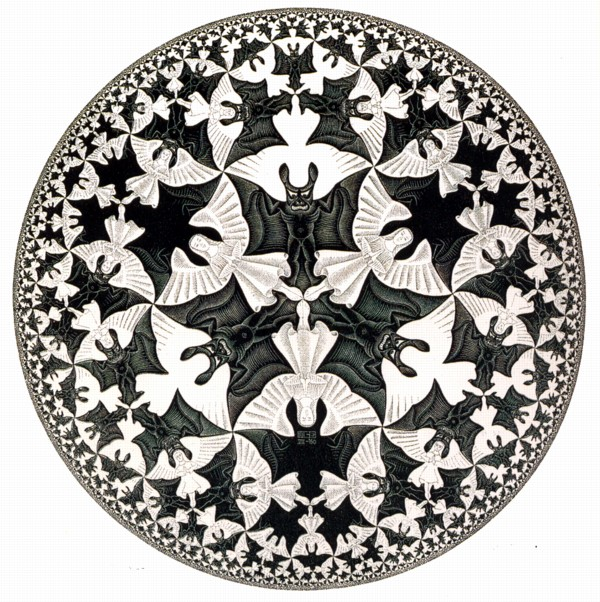
\includegraphics[width=0.6\textwidth]{C:/OneDriveSchool_Personal/OneDrive - Umich/Math/Classes/Winter_2022/History_of_Mathematics/Final/ME/Resources/Hyperbolic_Gemometry/Circle-limit-IV.jpg} \\
  Circle Limit IV \textbf{[3]} 
\end{center}

\section{Russell's Paradox}

\hspace{5mm}
In 1877 Cantor submitted to Crelle's Journal a paper bringing clarity to one to one correspondence, 
studying denumerable sets one to one with the natural numbers and sets of equal power, i.e. those one to one with each other. 
While Kronecker received the paper with suspicion, Dedekind supported the work of Cantor. 
In the following years from 1879 to 1884 Cantor published a series of six papers to Mathematische Annalen in which he provided a basic introduction to set theory. \textbf{[10]} 
In parallel, Frege published his first major work in 1879, presenting the a logical system quantifying negation implication, universality and in general, the ideas used to produce truth tables. 
Following these works Cantor suffered a bout of depression, coupled with mathematical doubts on his own work. 
Frege continued to develop a formal system of logic for arithmetic, publishing in 1892 Die Grundgestze der Arithmetik, Volume I. \textbf{[9]} 
In the midst of academic competition between the two, the development of today's naive set theory was born by combining Frege's logic with Cantor's sets. 

\hspace{5mm}
By 1895, Cantor discovered the first paradoxes in the theory of sets, soon after writing to Hilbert in 1896 with an explanation. 
Burali-Forti independently discovered such paradox then publishing his findings in 1897. 
At this point Cantor's works began to slow as life challenges address him and the depression continued. \textbf{[10]} 
As Frege had laid the ground work for the logical approach to natural numbers in his Volume I, he continued his work, extending his ideas to real numbers of which he was developing in Volume II. 
Then when in the state of publication of Volume II, Frege received a letter from Russell in 1902 pointing our the so called Russell's Paradox present in Volume I. 
The axiom at fault, originally introduced by Cantor, while leveraged by Frege, is the unrestricted comprehension (or abstraction) axiom. 
The axiom follows that any predicate expression on a free object determines the set of objects satisfying the predicate acting on the object. \textbf{[4]} 

\hspace{5mm}
The problem with unrestricted comprehension arises in the context a set of all sets which are not members of themselves. 
A common informal explanation follows from the set of all barbers who shave those men that do not shave themselves. 
For instance, consider such a barber that does not shave thyself, by the definition of the set, he must shave himself. 
As no barber in the set may shave thyself, we arrive at a logical contradiction. \textbf{[1]}
In a more formal consideration, take any set that is a member of itself, and now consider the set of sets that are not a member of themselves.
Well, if the set of sets which is not a member of thyself, is a member of itself then it is a member of itself. 
Similarly, if it is not a member of itself, than it itself must be a member of itself, both arriving at a contradiction. \textbf{[5]}
The letter from Russell initiated a correspondence with Frege, of which resulted in an appendix to Volume II with a modified axiom such to restore consistency. 
In this attempt, Frege faced additional conflict with his prior work, and was left with a still inconsistent system and a plethora of flash theorems existing within Volume I. \textbf{[9]} 
Russell responded to his own paradox with the introduction of the theory of types. 
He defined type as an intrinsic principal of sets, determined by the objects residing within them. \textbf{[4]}
One may think of basic set types being sets of base objects, sets of sets of base objects, and sets of sets of sets of base objects. 
The nesting present with the theory of types provides a natural hierarchical approach to the logic of sets. 
The work of Cantor and Frege to develop mathematical logic displays the disciplinary overlap present between mathematics and philosophy. 
It is worth noting at end now that the work of Cantor and Frege was not futile, but rather developed naive set theory. 
With the advent of Russell's paradox attention was drawn of which the modern axiomatic theories of sets and logic was born. 

\section{References}

\textbf{[1]} 
Baldwin, J. T., \& Lessmann, O. (1998). \textit{What is Russell's paradox?} Retrieved from \url{https://www.scientificamerican.com/article/what-is-russells-paradox/}

\textbf{[2]} 
Clair, B. (2016). \textit{Hyperbolic geometry,} Retrieved from \url{https://mathstat.slu.edu/escher/index.php/Hyperbolic_Geometry}

\textbf{[3]} 
Escher, M.C. (1960). \textit{Circle Limit IV,} (Heaven and Hell).

\textbf{[4]} 
Irvine, A. D. (1996). \textit{Bertrand Arthur William Russell - Biography,} Retrieved from \url{https://mathshistory.st-andrews.ac.uk/Biographies/Russell/}

\textbf{[5]} 
Irvine, A., \& Deutsch, H. (2020). \textit{Russell's paradox.} Retrieved from \url{https://plato.stanford.edu/entries/russell-paradox/}

\textbf{[6]} 
Keng, B. (2018). \textit{Hyperbolic geometry and Poincaré embeddings.} Retrieved from \url{https://bjlkeng.github.io/posts/hyperbolic-geometry-and-poincare-embeddings/}

\textbf{[7]} 
Knudson, K. (2011). \textit{A Gentle Introduction to Hyperbolic Geometry [PDF].} Gainesville: University of Florida George A. Smathers Libraries.

\textbf{[8]} 
Milnor, J.W. (1982). \textit{Hyperbolic geometry: The first 150 years.} Bulletin of the American Mathematical Society, 6, 9-24.

\textbf{[9]} 
O'Connor, J. J., \& Robertson, E. F. (2002). \textit{Friedrich Ludwig Gottlob Frege - Biography,} Retrieved from \url{https://mathshistory.st-andrews.ac.uk/Biographies/Frege/}

\textbf{[10]} 
O'Connor, J. J., \& Robertson, E. F. (1998). \textit{Georg Ferdinand Ludwig Philipp Cantor - Biography,} Retrieved from \url{https://mathshistory.st-andrews.ac.uk/Biographies/Cantor/}

\textbf{[11]} 
O'Connor, J. J., \& Robertson, E. F. (2000). \textit{Nikolai Ivanovich Lobachevsky - Biography,} Retrieved from \url{https://mathshistory.st-andrews.ac.uk/Biographies/Lobachevsky/}

\textbf{[12]} 
Stillwell, J. (2020). \textit{Mathematics and Its History: A Concise Edition.} (Undergraduate Texts in Mathematics). Springer, Cham.

\end{document}